\section{Introduction}
\label{sec:intro}

Knowledge distillation usually treats the teacher signal as a target to be matched uniformly: logits, features, or token embeddings are reconstructed with little regard for which parts of the representation support the teacher's decision.
For visual models, however, explanation methods provide an additional signal: they estimate which image regions or visual tokens were most influential for a prediction.
This raises the central research question of this work: \emph{can explainability provide a useful training signal for knowledge distillation, beyond ordinary feature reconstruction?}
We study this question in a demanding setting where the distilled visual encoder is not evaluated only by representation similarity, but is plugged back into a VLM and judged through the answers that the full system generates.
The plug-in VLM evaluation is therefore a stress test for the explanation-guided distillation signal: it asks whether saliency-weighted supervision preserves information that still matters after visual features are consumed by a language model.

We study this question with Qwen2.5-VL~\citep{qwen2025vl}.
The teacher VLM provides visual-token targets, and a ViT student~\citep{dosovitskiy2021image} is trained to replace the teacher's visual module while the language model is kept fixed.
The student is smaller than the original visual pathway, but compression is not the main scientific claim.
The main claim is about supervision: explanations may identify which parts of the teacher representation are most important to preserve for downstream generation.

The proposed supervision uses a teacher-side probe to produce Grad-CAM saliency over visual tokens~\citep{selvaraju2017gradcam}.
Instead of treating all token errors equally, the explanation-guided objective weights token reconstruction by saliency.
This converts an explanation into a training signal: the student is asked to prioritize teacher features that the probe identifies as decision-relevant.
The study compares this signal against plain global MSE and against combined global-plus-explanation objectives.

\begin{figure*}[t]
  \centering
  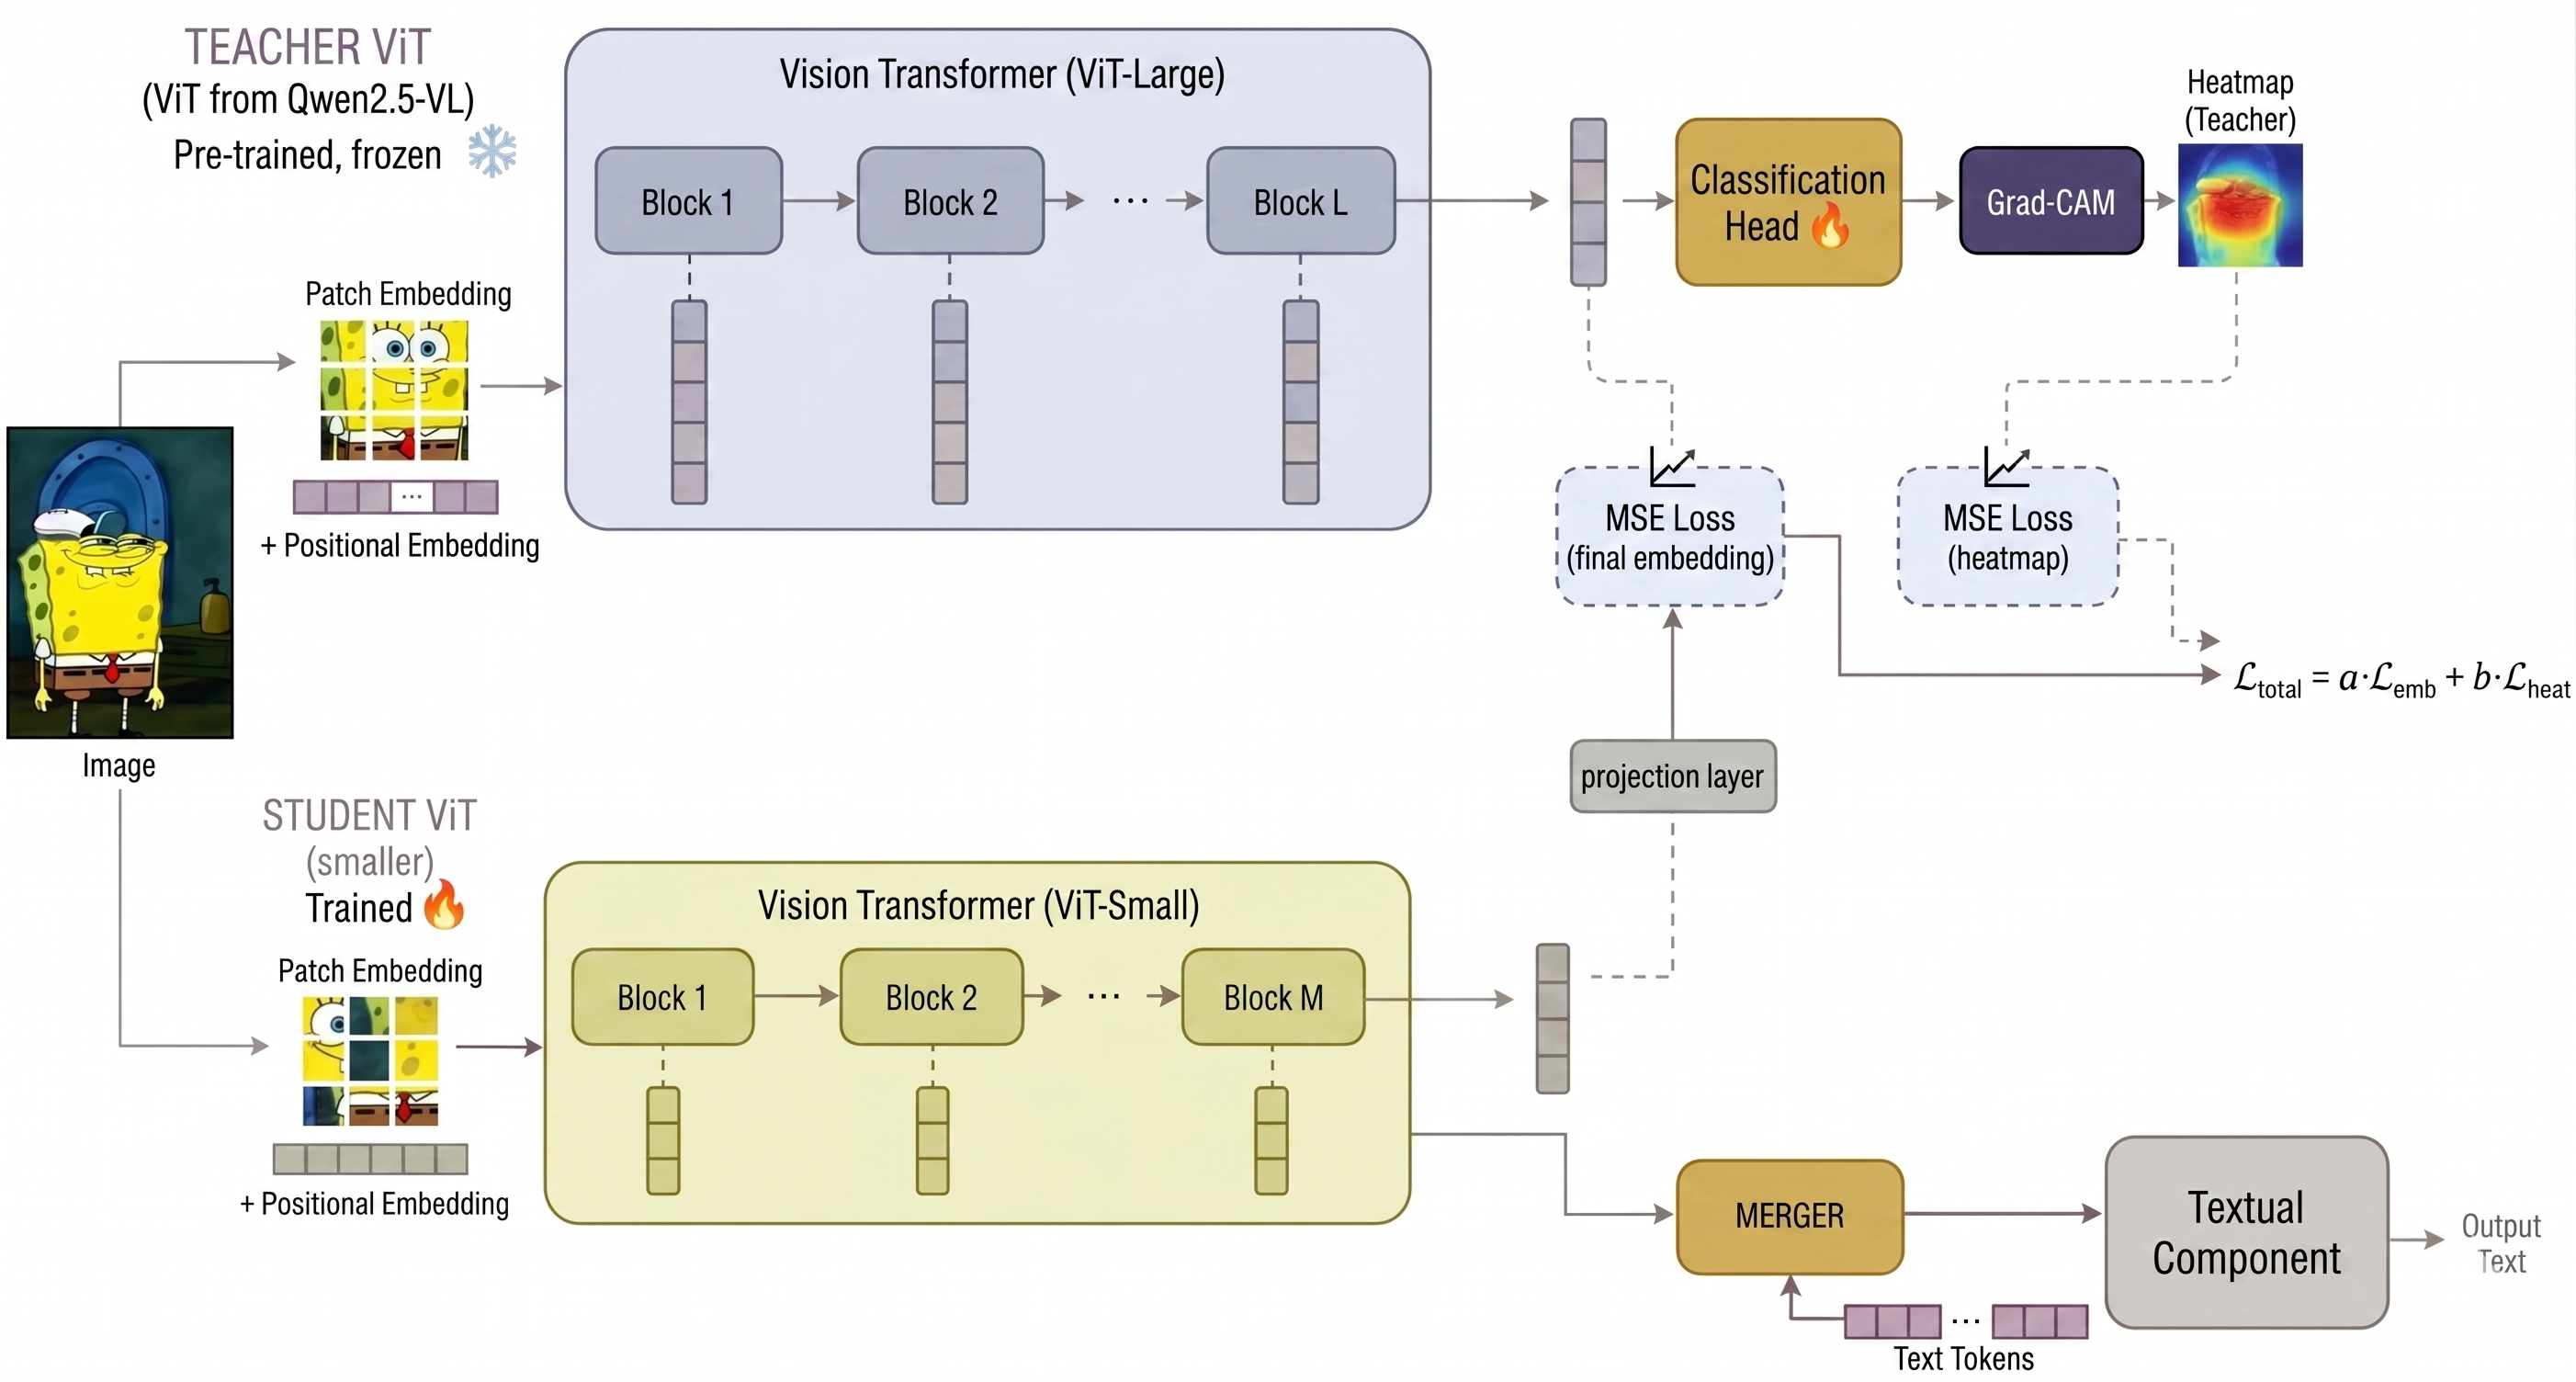
\includegraphics[width=0.96\textwidth]{figures/pipeline.png}
  \caption{Pipeline overview.}
  \label{fig:pipeline}
\end{figure*}

After distillation, each student visual encoder is inserted into the same VLM generation pipeline, and the resulting answers are compared with answers from the original teacher system.
Three independent VLM judges perform blind A/B comparisons while seeing the image, so the primary metric reflects image-grounded answer preference rather than embedding similarity or text overlap alone.

The original VLM is still preferred on most examples, but the ablation shows a consistent effect of the explanation signal.
Global MSE alone produces very few student-preferred answers, whereas saliency-weighted distillation consistently improves the student preference rate.
This pattern suggests that the saliency map is not merely a visualization artifact: used as a token-level weighting signal, it changes which teacher features the student preserves, and that change remains visible in downstream VLM behavior.

The remainder of the paper is organized as follows.
Section~\ref{sec:related} situates the work relative to VLMs, visual distillation, explanation-based supervision, and generated-answer evaluation.
Section~\ref{sec:method} describes the experimental setting, teacher-probe construction, explanation-guided distillation objective, and blind image-grounded judge protocol.
Section~\ref{sec:results} reports probe quality, downstream VLM preference results, judge tendencies, and qualitative answer patterns.
Sections~\ref{sec:limitations} and~\ref{sec:conclusion} summarize the main limitations and conclusions.

\section{Related Work}
\label{sec:related}

\paragraph{Vision-language models.}
Qwen2.5-VL is an open VLM family designed for visual perception, grounding, document understanding, and instruction following~\citep{qwen2025vl}.
This work treats the VLM as the downstream system in which a distilled visual module must operate. Keeping the language model, and the merger module, fixed isolates the question of whether visual-module distillation preserves useful image evidence.
Large VLMs build on a line of work that aligns visual encoders with language supervision and then connects visual representations to text decoders or instruction-following language models.
CLIP showed that natural-language supervision can train transferable visual representations at scale~\citep{radford2021clip}.
Later architectures such as BLIP-2 and LLaVA made the interface between a visual encoder and a frozen or instruction-tuned language model a central design object~\citep{li2023blip2,liu2023llava}.
Our setting evaluates the student inside the VLM rather than treating the visual encoder as an isolated classifier.

\paragraph{Knowledge distillation.}
Knowledge distillation trains a student model to reproduce information carried by a stronger teacher~\citep{hinton2015distilling}.
The original formulation uses softened class probabilities, making the teacher provide a richer target than one-hot labels.
Subsequent work broadened the teacher signal beyond output logits: FitNets introduced intermediate feature hints, while attention transfer used spatial attention maps as structured supervision~\citep{romero2015fitnets,zagoruyko2017attention}.
These methods show that distillation can depend strongly on which teacher information is transferred, not only on the capacity of the student.
Our work follows this line but changes the role of the auxiliary signal.
Instead of asking the student to match an attention or explanation map directly, we use explanation weights to decide where token-level feature reconstruction should matter most.
The question is therefore not only whether a student can imitate a teacher, but whether an explainability-derived weighting of the teacher signal improves what the student preserves.

\paragraph{Explanations as supervision.}
Grad-CAM uses gradients to identify image regions that support model decisions~\citep{selvaraju2017gradcam}.
In this work, saliency is not only a post-hoc visualization.
It weights the token-level distillation loss, turning explanations into a selective supervision signal.
This connects to attention-transfer work, where spatial or channel-wise attention patterns are used as additional supervision for a student~\citep{zagoruyko2017attention}.
The difference is that our signal is class-conditioned and produced from a teacher-side probe over VLM visual tokens.
Rather than asking the student to reproduce an explanation map directly, we use the saliency map acting as a signal: relevant tokens should be more expressive than tokens with low estimated relevance.
